\LectureAnswerSection\subsection*{两级提示}
\phantomsection\label{hint:at1:drill:1}
\LectureHint{at1:drill:1}{先从平抛时间消去当地重力。}{用质量比与重力比求半径比的平方。}
\phantomsection\label{hint:at1:drill:2}
\LectureHint{at1:drill:2}{两次高度相同，重力比等于时间比的平方反比。}{先取正平方根，注意并不需要额外展开。}
\phantomsection\label{hint:at1:drill:3}
\LectureHint{at1:drill:3}{用质心矢量关系合并另外两颗星的引力。}{三个顶点得到相同的加速度与位置比例系数。}
\phantomsection\label{hint:at1:drill:4}
\LectureHint{at1:drill:4}{先减去月球对地心的共同加速度。}{保留小位移的一阶项，区分平移系与转动系。}
\phantomsection\label{hint:at1:drill:5}
\LectureHint{at1:drill:5}{同时考虑新增液体质量和离球心距离增大。}{对 $GM(r)/r^2$ 求导，而不是只改分母。}
\phantomsection\label{hint:at1:drill:6}
\LectureHint{at1:drill:6}{球内引力正比于有向位置。}{用表面静止的初值确定余弦相位。}
\phantomsection\label{hint:at1:drill:7}
\LectureHint{at1:drill:7}{外侧场同向，只在中间寻找零点。}{分别考察沿线和横向的场变化。}
\phantomsection\label{hint:at1:drill:8}
\LectureHint{at1:drill:8}{按薄壳逐层加入，而非使用表面势乘全部质量。}{装配过程中每一对只计一次。}
\phantomsection\label{hint:at1:drill:9}
\LectureHint{at1:drill:9}{将质量写成平均密度乘体积。}{比较周期与线速度时保留各自的半径因子。}
\phantomsection\label{hint:at1:drill:10}
\LectureHint{at1:drill:10}{承接腔内均匀场，但本题新增自由运动与壁面边界。}{从腔心到靠近原球心的一侧壁面位移为腔半径。}
\Needspace{8\baselineskip}\subsection*{详解}
\begin{drillsolution}{at1:drill:1}
图\ref{fig:at1:drill:1:s} 表示每个星球自己的局部平抛，飞行时间 $t_i=\sqrt{2h_i/g_i}$，故 $x_i=v_it_i$，解得 $g_i=2h_iv_i^2/x_i^2$。
\typeout{ASTROFIG:fig:at1:drill:1:p}\fig{fig:at1:drill:1:p}{解答过程：平抛测量给出的半径比}{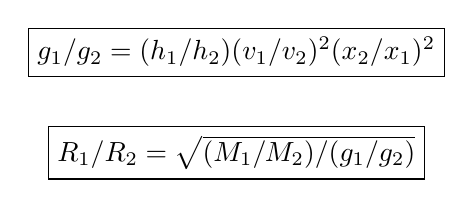
\begin{tikzpicture}[scale=.85]
\node[draw]at(0,1){$g_1/g_2=(h_1/h_2)(v_1/v_2)^2(x_2/x_1)^2$};\node[draw]at(0,-.5){$R_1/R_2=\sqrt{(M_1/M_2)/(g_1/g_2)}$};
\end{tikzpicture}}

图\ref{fig:at1:drill:1:p} 的比例式给
\[\frac{g_1}{g_2}=\frac65\left(\frac87\right)^2\left(\frac43\right)^2=\frac{2048}{735}.
\]
再由 $g_i=GM_i/R_i^2$，
\[\frac{R_1^2}{R_2^2}=\frac{M_1/M_2}{g_1/g_2}=\frac{1225}{4096},\qquad R_1:R_2=35:64.\]
半径取正根。局部平抛近似要求下落高度和射程相对星球半径足够小，否则重力大小及方向的变化都要计入。\end{drillsolution}
\begin{drillsolution}{at1:drill:2}
图\ref{fig:at1:drill:2:s} 两次实验的当地重力分别为 $2h/t^2$ 和 $2h/(t+\Delta t)^2$。与平方反比式比较，
\[\frac{g_H}{g_0}=\left(\frac{t}{t+\Delta t}\right)^2
=\left(\frac{R}{R+H}\right)^2.
\]
\typeout{ASTROFIG:fig:at1:drill:2:p}\fig{fig:at1:drill:2:p}{解答过程：由落下时间差估计山高}{\begin{tikzpicture}[scale=.85]
\draw[world](0,0)--(3,0);\draw[world](0,1.8)--(3,1.8);\node[left]at(0,0){$R$};\node[left]at(0,1.8){$R+H$};\draw[flow](1,2.6)--(1,2)node[right]{$t+\Delta t$};\draw[flow](2,.8)--(2,.2)node[right]{$t$};
\end{tikzpicture}}

图\ref{fig:at1:drill:2:p} 中时间和半径均为正，直接开平方得 $(t+\Delta t)/t=(R+H)/R$，所以 $H=R\Delta t/t$。在“各次短下落内重力恒定”的模型中它已经是精确代数关系；不必再对平方式作一次重复近似。实际应用仍要求 $h\ll R,R+H$，且自转、空气阻力等影响可以忽略。\end{drillsolution}
\begin{drillsolution}{at1:drill:3}
图\ref{fig:at1:drill:3:s} 的三条边长度相同，令质心为原点、位置为 $\bm r_i$，则 $\sum m_i\bm r_i=0$。对第一颗星，
\[\ddot{\bm r}_1=\frac G{l^3}\big[m_2(\bm r_2-\bm r_1)+m_3(\bm r_3-\bm r_1)\big]
=-\frac{G(m_1+m_2+m_3)}{l^3}\bm r_1.
\]
\typeout{ASTROFIG:fig:at1:drill:3:p}\fig{fig:at1:drill:3:p}{解答过程：正三角形三体的共同转动}{\begin{tikzpicture}[scale=.85]
\draw[world](0,0)--(4,0)--(2,3.464)--cycle;\fill(2.5,1.5)circle(2pt)node[right]{$C$};\draw[force](0,0)--(1,.6);\draw[force](4,0)--(3.4,.6);\draw[force](2,3.464)--(2.25,2.48);
\end{tikzpicture}}

图\ref{fig:at1:drill:3:p} 显示合加速度指向真正的质心 $C$，另外两颗星循环换下标得到同样系数。因此统一取 $\omega^2=G(m_1+m_2+m_3)/l^3$，便满足三个向心方程。质量不等时质心一般不是几何中心，但这个证明仍成立。存在共同转动解不等于它对任意扰动都稳定，本题没有证明稳定性。\end{drillsolution}
\begin{drillsolution}{at1:drill:4}
图\ref{fig:at1:drill:4:s} 的原点本身受月球加速度 $g_O=GM'/D^2$，必须先扣除。沿连线的差为
\[\Delta g_A=GM'\left[\frac1{(D-x)^2}-\frac1{D^2}\right]
\simeq\frac{2GM'x}{D^3},\]
指向 $+x$。
\typeout{ASTROFIG:fig:at1:drill:4:p}\fig{fig:at1:drill:4:p}{解答过程：近侧与横向的潮汐加速度}{\begin{tikzpicture}[scale=.85]
\draw[axis](-1,0)--(7,0)node[right]{$x$};\draw[axis](0,-.6)--(0,5)node[above]{$y$};\draw[force](4,0)--(6,0)node[midway,below]{$2GM^\prime x/D^3$};\draw[force](0,4)--(0,2)node[midway,left]{$GM^\prime y/D^3$};\node[right]at(0,4){$B$};\node[above]at(4,0){$A$};
\end{tikzpicture}}

图\ref{fig:at1:drill:4:p} 对 $B$ 的月球场为 $GM'(D,-y)/(D^2+y^2)^{3/2}$。其 $x$ 分量与原点的差为二阶，$y$ 分量保留一阶得 $-GM'y/D^3$，故横向向地月连线压缩。若题目改用转动坐标系，应另外加入该参考系的离心、科里奥利作用；本题已明确不转动，不能凭空多加一个离心梯度。\end{drillsolution}
\begin{drillsolution}{at1:drill:5}
图\ref{fig:at1:drill:5:s} 液层底部的包围质量为 $M$。向上增加 $\dd r$ 时，包围质量增加 $4\pi R^2\rho\dd r$，而距离平方也改变。
\typeout{ASTROFIG:fig:at1:drill:5:p}\fig{fig:at1:drill:5:p}{解答过程：薄液层内近似不变的重力}{\begin{tikzpicture}[scale=.85]
\node[draw]at(0,1){包围质量增加：$+4\pi R^2\rho\dd r$};\node[draw]at(0,-.5){距离增大：$-2GM\dd r/R^3$};
\end{tikzpicture}}

按 图\ref{fig:at1:drill:5:p} 的两种变化同时求导：
\[g'(R)=G\left[\frac{4\pi R^2\rho}{R^2}-\frac{2M}{R^3}\right]=0,
\qquad\rho=\frac{M}{2\pi R^3}=\frac23\bar\rho_M.
\]
若要求有限厚度范围中 $g(r)=g_c$ 严格不变，则 $M(r)=g_cr^2/G$，求导得 $\rho(r)=g_c/(2\pi Gr)$，并不严格均匀。因此常密度答案是在 $h/R$ 小量下抵消一阶变化，不应夸大为任意厚度的精确结果。\end{drillsolution}
\begin{drillsolution}{at1:drill:6}
图\ref{fig:at1:drill:6:s} 沿隧道取有向坐标 $x$，球内场给 $\ddot x=-GMx/R^3$，并非恒定加速度。
\typeout{ASTROFIG:fig:at1:drill:6:p}\fig{fig:at1:drill:6:p}{解答过程：均匀星球的直径隧道}{\begin{tikzpicture}[scale=.85]
\draw[axis](-.2,0)--(4.5,0)node[right]{$t$};\draw[axis](0,-.2)--(0,2.4)node[above]{$x$};\draw[world,domain=0:4.1,samples=90]plot(\x,{1.6*cos(90*\x)});\node at(2.6,2){$x=R\cos\omega t$};
\end{tikzpicture}}

图\ref{fig:at1:drill:6:p} 的初值 $x(0)=R,\dot x(0)=0$ 选定 $x=R\cos\omega t$，$\omega=\sqrt{GM/R^3}$。第一次过球心满足 $\omega t=\pi/2$，时间 $\pi/(2\omega)$；到另一端满足 $\omega t=\pi$，时间 $\pi/\omega$。全振动周期 $2\pi\sqrt{R^3/(GM)}$ 等于近表面理想圆轨道周期。该比较是两个不同模型的数学巧合，不能把隧道运动误认为圆周运动。\end{drillsolution}
\begin{drillsolution}{at1:drill:7}
  图\ref{fig:at1:drill:7:s} 外侧两场同向，零点只能在两质量之间。令距 $M_1$ 为 $x$，有 $GM_1/x^2=GM_2/(L-x)^2$，取正根得 $x=L\sqrt{M_1}/(\sqrt{M_1}+\sqrt{M_2})$。
  \typeout{ASTROFIG:fig:at1:drill:7:p}\fig{fig:at1:drill:7:p}{解答过程：两固定天体之间的零场点}{\begin{tikzpicture}[scale=.85]
\fill(0,0)circle(3pt)node[above]{$M_1$};\fill(5,0)circle(3pt)node[above]{$M_2$};\draw[dim](0,-.6)--(5,-.6)node[midway,below]{$L$};\fill(2.8,0)circle(2pt)node[below]{$P$};\draw[force](3,.3)--(3.8,.3);\draw[force,blue](2.8,1.2)--(2.8,.5);
\end{tikzpicture}}

  图\ref{fig:at1:drill:7:p} 沿线场分量 $g_x=-GM_1/x^2+GM_2/(L-x)^2$，导数 $2GM_1/x^3+2GM_2/(L-x)^3>0$，故向右扰动产生向右场，沿线不稳定。横向小位移 $y$ 时，两质量都产生向连线的分量，$g_y\simeq-G[M_1/x^3+M_2/(L-x)^3]y$，横向有恢复作用。局部横向恢复不等于三维整体稳定，这个点是鞍型平衡。\end{drillsolution}
\begin{drillsolution}{at1:drill:8}
  图\ref{fig:at1:drill:8:s} 已装入半径 $r$ 的球，质量 $M(r)=Mr^3/R^3$。新增薄壳 $\dd M=3Mr^2\dd r/R^3$，它与已有内球的能量增量为 $\dd U=-GM(r)\dd M/r$。
  \typeout{ASTROFIG:fig:at1:drill:8:p}\fig{fig:at1:drill:8:p}{解答过程：均匀球的自引力能}{\begin{tikzpicture}[scale=.85]
\draw[flow](0,0)--(4,0);\node[above]at(0,0){$M(r)$};\node[above]at(4,0){$M(r)+\dd M$};\node at(2,-1){$\dd U=-GM(r)\dd M/r$};
\end{tikzpicture}}

  图\ref{fig:at1:drill:8:p} 从零半径装到 $R$，
  \[U=-\frac{3GM^2}{R^6}\int_0^Rr^4\dd r=-\frac{3GM^2}{5R}.
  \]
  把各部分分散至无穷远且末态无剩余动能，需增加势能到零，最少功 $3GM^2/(5R)$。过程已让每对质量只计算一次，不能再乘一半。若题目为压缩到 $R/2$ 且保持均匀，则能量下降 $3GM^2/(5R)$，这部分可转成热或辐射，而不应凭空消失。\end{drillsolution}
\begin{drillsolution}{at1:drill:9}
  图\ref{fig:at1:drill:9:s} 每颗星球的 $M=4\pi\rho R^3/3$，圆轨道半径取 $R$ 的极限。代入 $T^2=4\pi^2R^3/(GM)$，所有 $R^3$ 消去，得
  \[T=\sqrt{\frac{3\pi}{G\rho}},\qquad \rho=\frac{3\pi}{GT^2}.
  \]
  \typeout{ASTROFIG:fig:at1:drill:9:p}\fig{fig:at1:drill:9:p}{解答过程：同密度星球的近表面周期}{\begin{tikzpicture}[scale=.85]
\node[draw]at(0,1){$M\propto R^3$};\node[draw]at(0,-.5){$T^2\propto R^3/M$：半径抵消};
\end{tikzpicture}}

  图\ref{fig:at1:drill:9:p} 表明相同密度给相同周期，但线速度 $\sqrt{GM/R}=R\sqrt{4\pi G\rho/3}$ 随半径增加。周期相同不等于速度相同。真实卫星必须在表面外，若高度不可忽略，推密度时还应乘 $(r/R)^3$，不能把整个轨道半径误作星球半径。\end{drillsolution}
\begin{drillsolution}{at1:drill:10}
  图\ref{fig:at1:drill:10:s} 的均匀腔内场为 $\bm g_c=-4\pi G\rho\overrightarrow{OC}/3$，大小 $g_c=2\pi G\rho R/3$。物体沿 $C$ 指向 $O$ 直线运动，先到达靠近 $O$ 的腔壁，位移为腔半径 $R/2$。
  \typeout{ASTROFIG:fig:at1:drill:10:p}\fig{fig:at1:drill:10:p}{解答过程：空腔内自由运动的到达时间}{\begin{tikzpicture}[scale=.85]
\draw[world](0,0)--(3,0);\fill(2,0)circle(2pt)node[above]{$C$};\fill(0,0)circle(2pt)node[above]{腔壁};\draw[force](2,.5)--(.8,.5)node[above]{$g_c$};\draw[dim](0,-.5)--(2,-.5)node[midway,below]{$R/2$};
\end{tikzpicture}}

  图\ref{fig:at1:drill:10:p} 在到壁前加速度恒定，$R/2=g_ct^2/2$，所以 $t=\sqrt{3/(2\pi G\rho)}$，速度 $v=g_ct=R\sqrt{2\pi G\rho/3}$。到达壁面后需加入接触条件，不能继续把自由运动抛物线延伸进实体。时间不含 $R$，因为位移与加速度都正比于半径；速度仍正比于 $R$。\end{drillsolution}
